\begin{enumerate}
	\item 
اگر $D$ و $K$ را با بردار جایگزین کنیم (با توجه به این که قطری هستند)، داریم
$A_{i,:} = d_i + k_iG_{i,:}$.
همچنین
\[
\gamma tr(D^{-1}) + tr(K^{-1}) = \sum \frac{\gamma}{d_i} + \sum \frac{1}{k_i}
\]
با این توصیفات مساله به فرم زیر در مي‌آید.\\
\[
minimize \quad \lambda_{max}(A)
\]\[
s.t. \quad d \ge 0 \land k \ge 0\]\[
A_{i,:} = d_i + k_iG_{i,:}\]\[
\sum \frac{\gamma}{d_i} + \sum \frac{1}{k_i} \le u
\]
که با توجه به محدب بودن بزرگترین مقدار ویژه و نیز $\frac{1}{x}$، مساله به فرم مناسب درآمد.
%به وضوح مساله محدب است چون
%$\lambda_{max}$
%یک تابع محدب است زیرا می‌توان آن را به فرم زیر نوشت
%\[
%sup_{\{x: ||x||\le 1\}} \quad ||Ax||
%\]
%نوشت.
\item 
کد مورد نظر در زیر (و مجددا در صورتی که نیاز باشد در فایل $q6$ آمده است) خروجی هم در شکل
\ref{fig:6}
قابل مشاهده است.
\begin{latin}
	\lstinputlisting[breaklines]{../code/q6.py}
\end{latin}
\begin{figure}[H]
	\centering
	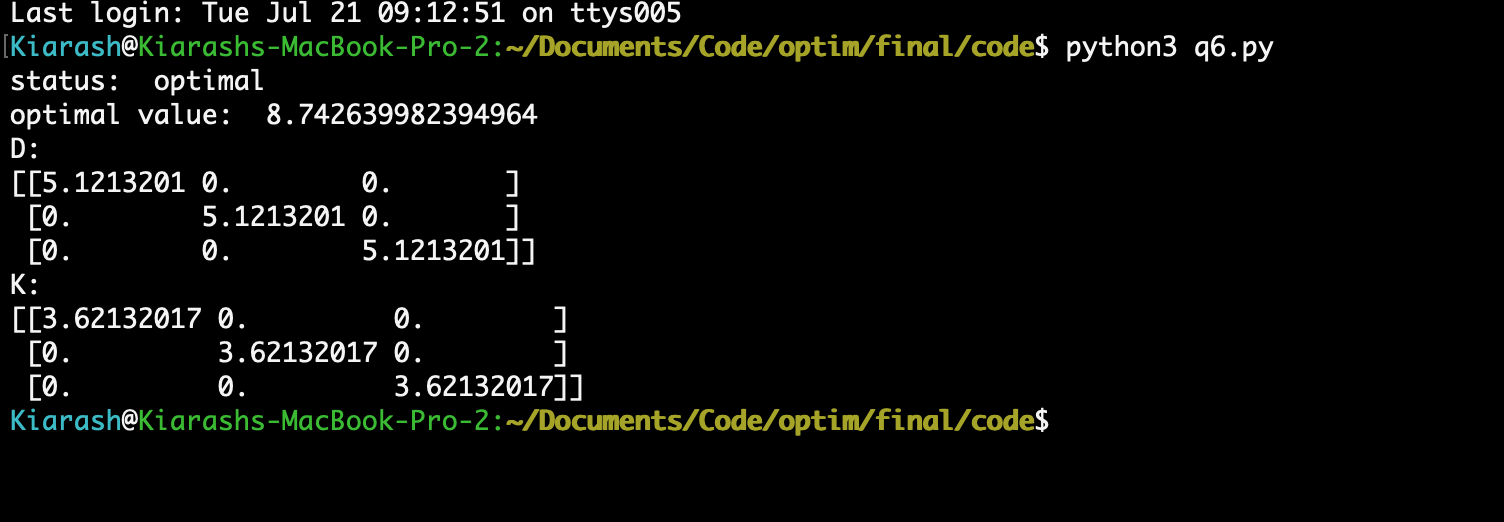
\includegraphics[width=0.9\textwidth]{q6}
	\caption{شکل سوال 6}
	\label{fig:6}
\end{figure}
\textbf{در صورتی که استدلال فوق به علت فرض تقارن نمره‌ی خاصی نمی‌گیرد}:
نتونستم مساله رو حل کنم اما خب تنها چیزی که ذهنم رسید رو می‌نویسم. استاد گفتند که $A$ ماتریس دلخواه نیست. به این منظور کافیه دقت کنیم که اگه معادله‌ی مقدارویژه و بردار ویژه رو در نظر بگیریم، میشه به این شکل بهش نگاه کرد (میشه فرم بلوکی هم نوشت اینو که خب فرقی نمی‌کنه صرفا همین معادله‌هست)
\[
Gv = y, \quad Dv + Ky = \lambda v
\]
%\textbf{در صورتی که استدلال فوق اشتباه است:}
%\footnote{
%در واقع من مقدار تکین را کمینه کرده‌ام و نه مقدارویژه را. این که یکی هستند یا نه را نمی‌دانم. در هر حال، در حالت کلی، یک راه حل
%\lr{quasiconvex}
%وجود دارد که آن را توضیح می‌دهم. با توجه به مطالبی که در سوال ۱ گفته شده بود، نمی‌دانم که 
%\lr{quasiconvex}
%هم اوکی است یا نه و برای همین می‌نویسم تا شاید نمره‌ای بگیرم.
%با توجه به زمان هم فکر نکنم بتوانم از استاد در کوئرا بپرسم (الان ۹ و نیم صبحه). اگر دید تیم تصحیح این است که دارم ۲ تا جواب می‌نویسم و قرار است بین ۲ تا جواب مینممم بگیرید یعنی به ضرر من عمل کنید، همان جواب اولی را در نظر بگیرید یعنی
%فرمول‌بندی
%\lr{convex}
%اما خب با مقدار تکین. ولی خب لطفا این رو هم بخونید چون جالبه.
%}
%دقت کنید که اگر 
%$\lambda$
%را بتوان تولید کرد، با ضرب
%$K, D$
%در یک اسکالر بزرگتر از ۱، چون شرط
%کران‌بالا که خراب نمی‌شود، می‌توان هر ضریب بزرگتر از ۱ای از لامبدا را هم تولید کرد.
%از طرفی اگر 
%$\lambda$
%را بدانیم، بررسی این که آیا $D, K$ مناسب یافت می‌شوند یا نه، 
\end{enumerate}